\documentclass[xcolor=table]{beamer}
\usepackage{lmodern}
%\usepackage[normalem]{ulem}
\usepackage{ marvosym }
\usepackage[export]{adjustbox}
\usepackage{mathtools,calc}
\newcommand\Fontvi{\fontsize{22}{23.2}\selectfont}
\newcommand\strikeout[2][]{%
 \begin{tabular}[b]{@{}c@{}}
    \makebox(0,0)[cb]{\textcolor{blue}{#1}} \\[-0.2\normalbaselineskip]
     \rlap{\color{red}\rule[0.5ex]{\widthof{#2}}{0.5pt}}#2
 \end{tabular}}

\newcommand<>\mathalt[2]{%
  \alt#3{\mathmakebox[\widthof{$#2$}]{#1}}{#2}%
}
\usepackage{colortbl}
\usepackage{booktabs}
%\usepackage{xcolor}
%\usepackage[usenames, dvipsnames]{color}
\definecolor{red}{rgb}{0.894, 0.101, 0.109} 
\definecolor{Gray}{gray}{0.85}
\newcolumntype{a}{>{\columncolor{Gray}}c}
\definecolor{green}{rgb}{0.1054, 0.6171, 0.4648}
\definecolor{orange}{rgb}{0.8476, 0.3711, 0.0078}
\definecolor{violet}{rgb}{0.9023, 0.1602, 0.5391}
%\usepackage[doi=false, backref=true, url=false, isbn=false, backend=biber,
						%citestyle=authoryear]{biblatex}
\usepackage{tabu}
\newcommand{\blue}{\textcolor{blue}}
\newcommand{\red}{\textcolor{red}}
\newcommand{\green}{\textcolor{green}}
\newcommand{\organge}{\textcolor{orange}}
\newcommand{\violet}{\textcolor{violet}}
% Just for demo

\AtBeginSection[]{
  \begin{frame}
  \vfill
  \centering
  \begin{beamercolorbox}[sep=8pt,center,shadow=true,rounded=true]{title}
    \usebeamerfont{title}\insertsectionhead\par%
  \end{beamercolorbox}
  \vfill
  \end{frame}
}
\usepackage{mathtools}
\newtheorem{prop}{Proposition}
\newtheorem{hypothesis}{Hypothesis}
\usepackage{amsmath}
\usepackage{multirow}
\usepackage{makecell} % to make linebreaks in table
\renewcommand\theadalign{bc}
\renewcommand\theadfont{\bfseries}
\renewcommand\theadgape{\Gape[4pt]}
\renewcommand\cellgape{\Gape[4pt]}
\usepackage{hhline}
\usepackage{geometry}
\usepackage{booktabs}
\usepackage[]{hyperref}%
\hypersetup{colorlinks, linkcolor={blue}, citecolor={blue}, urlcolor={red}}
\usepackage{graphicx}

\DeclareMathOperator*{\argmax}{\arg\!\max}
\DeclareMathOperator{\E}{\mathbb{E}}
%\addbibresource[]{library.bib}
\usepackage[utf8]{inputenc}
\usepackage[T1]{fontenc}
\setbeamertemplate{caption}{\raggedright\insertcaption\par}
\usetheme{default}
\usepackage[flushleft]{threeparttable}
\usepackage{booktabs,caption,fixltx2e}
\usepackage{ragged2e}
\usepackage{appendixnumberbeamer}
\makeatletter
\usefonttheme{professionalfonts}
\usefonttheme{serif}
\setbeamertemplate{navigation symbols}{}%remove navigation symbols
\setbeamertemplate{footline}
{
  \leavevmode%
  \hbox{%
  \begin{beamercolorbox}[wd=.333333\paperwidth,ht=2.25ex,dp=1ex,center]{author in head/foot}%
    \usebeamerfont{author in head/foot}\insertsection\
  \end{beamercolorbox}%
  \begin{beamercolorbox}[wd=.333333\paperwidth,ht=2.25ex,dp=1ex,center]{title in head/foot}%
    \usebeamerfont{title in head/foot}\insertsubsection\
  \end{beamercolorbox}%
  \begin{beamercolorbox}[wd=.333333\paperwidth,ht=2.25ex,dp=1ex,right]{date in head/foot}%
    %\usebeamerfont{date in head/foot}\insertshortdate{}\hspace*{2em} % hide %date
    %\insertframenumber{} / \inserttotalframenumber\hspace*{2ex} 
  \end{beamercolorbox}}%
  \vskip0pt%
}
\makeatother
%\setbeamertemplate{footline}[frame number]{}


\usepackage{listings}
\lstset{
    tabsize=4,
    showstringspaces=false,
    numbers=left,
    commentstyle=\color{green},
    keywordstyle=\color{blue},
    stringstyle=\color{red}
}


 %----------------------------------------------------------------------------------------
% %	TITLE PAGE
% %----------------------------------------------------------------------------------------
\renewcommand*{\thefootnote}{\fnsymbol{footnote}}
\title[]{Mergesort with CUDA}
\date{25.02.2020} % Date, can be changed to a custom date
%\author{Fabian Schuetze, EUI}
\addtobeamertemplate{block begin}{}{\justifying}  %new code
\setbeamertemplate{itemize items}[circle]

\usepackage{tikz, enumitem}
\usetikzlibrary{positioning}% for positioning of nodes
\usetikzlibrary{decorations.pathreplacing,positioning, arrows.meta}
\newcommand{\ImageWidth}{11cm}


\begin{document}

\begin{frame}
\titlepage
\end{frame}

\section{Basic Architecture}

\begin{frame}
    \frametitle{Big Ideas}
    SMID, No fancy stuff, Latency Hiding. Can I show that?
\end{frame}

\begin{frame}[fragile]
\frametitle{GPU and CPU uses different memories}
\green{Basic Architecture:}
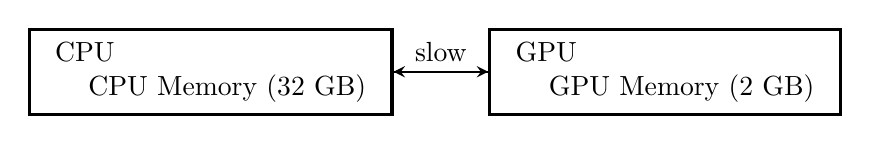
\begin{tikzpicture}[
node distance = 0mm and 12mm,% for distance between nodes
   box/.style = {draw, very thick, minimum width=5em},
      arrow/.style = {thick,-stealth}
                        ]
\node (n1) [box] {\begin{tabular}{ll}% text in nodes write as table
                  \multicolumn{2}{l}{CPU}   \\
                  &CPU Memory (32 GB)
                 \end{tabular}};
\node (n2) [box, below right=of n1.north east]
                {\begin{tabular}{ll}
                  \multicolumn{2}{l}{GPU}   \\
                    &GPU Memory (2 GB)
                 \end{tabular}};
\draw [arrow] (n1) --node [midway,above ] {slow} (n2);
\draw [arrow] (n2) -- (n1);
\end{tikzpicture}
\green{Memory Creation:}
\begin{lstlisting}[language=c++]
T* gpu_pointer;
unsigned int nBytes = 10*sizeof(int);
cudaMalloc((void**)&_gpu_pointer, nBytes);
\end{lstlisting}
\green{Memory Transfer:}
\begin{lstlisting}[language=c++]
cudaMemcpy(_gpu_pointer, _cpu_pointer, nBytes, cudaMemcpyHostToDevice));
\end{lstlisting}
\end{frame}

\begin{frame}[fragile]
\frametitle{Ideas for Memory Management}
\begin{lstlisting}[language=c++]
template <typename T>
class Storage {
   public:
    explicit Storage(const std::vector<T>&);

   private:
    std::vector<T> _data;
    T* _cpu_pointer;
    T* _gpu_pointer;
    void initialize_gpu_memory();
};
\end{lstlisting}
\begin{itemize}
    \item Memory pool, takes ownership
    \item Initializes the gpu memory as copy
    \item Pointers for cpu/gpu locations
\end{itemize}
\end{frame}

\begin{frame}[fragile]
    \frametitle{Lazy Memory Sync}
\begin{lstlisting}[language=c++]
class Storage {
   public:
    T* cpu_pointer();
    T* gpu_pointer();
    const T* cpu_pointer_const();
    const T* gpu_pointer_const();

   private:
    std::string head;
    void sync_to_cpu();
    void sync_to_gpu();
};
\end{lstlisting}
\begin{itemize}
    \item accesses const or non-const pointers
    \item $\text{head} \in \lbrace \text{CPU}, \text{GPU}, \text{SYNC} \rbrace $
    \item if non-const function: change $\text{head}$  to location
    \item Lazily sync if required pointer $!= \text{head}$
\end{itemize}
\end{frame}

\begin{frame}[fragile]
\frametitle{Launching CUDA threads}
    \green{Cuda Program}
\begin{lstlisting}[language=c++]
dim3 Grid(2)
dim3 Block(4)
add_kernel<<<Grid, Block>>>(...)
\end{lstlisting}
    \green{Thread Layout:}
    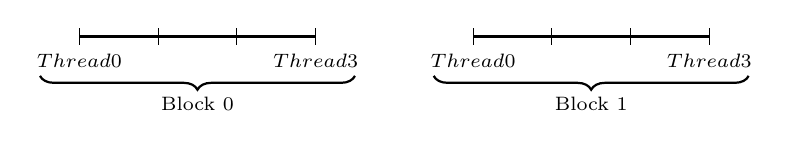
\begin{tikzpicture}
% draw horizontal line
\draw[thick,- ] (0,0) -- (3,0) node[font=\scriptsize,below left=3pt and
        -5pt]{};
\draw[thick,- ] (5,0) -- (8,0) node[font=\scriptsize,below left=3pt and
        -5pt]{};


% draw vertical lines
\foreach \x in {0,1,...,3}
\draw (\x cm,3pt) -- (\x cm,-3pt);

\foreach \x in {5,6,...,8}
\draw (\x cm,3pt) -- (\x cm,-3pt);

\foreach \x/\descr in {0/Thread 0,3/Thread 3}
\node[font=\scriptsize, text height=1.75ex,
text depth=.5ex] at (\x,-.3) {$\descr$};

\foreach \x/\descr in {5/Thread 0,8/Thread 3}
\node[font=\scriptsize, text height=1.75ex,
text depth=.5ex] at (\x,-.3) {$\descr$};

\draw [thick ,decorate,decoration={brace,amplitude=5pt}] (3.5,-0.5)  -- +(-4,0) 
       node [black,midway,below=4pt, font=\scriptsize] {Block 0};
\draw [thick ,decorate,decoration={brace,amplitude=5pt}] (8.5,-0.5)  -- +(-4,0) 
       node [black,midway,below=4pt, font=\scriptsize] {Block 1};
    \end{tikzpicture}
    \green{Addition:}
\begin{lstlisting}[language=c++]
__global__ 
add_kernel(float* A, float* B, float* C, int n) {
    int i = blockDim.x * blockIdx.x + threadIdx.x;
    if (i < n) {
        C[i] = A[i] + B[i];
    }
}
\end{lstlisting}

\end{frame}

\section{Merge}

\begin{frame}[fragile]
    \frametitle{Basic Merge Operation}
\begin{align*}
    A &= \begin{matrix} 5 7 8 9 12 14 15 16 \end{matrix} \\
    B &= \begin{matrix} 1 2 3 4 6 10 11 13 \end{matrix} \\
    C &= \begin{matrix} ? ? ? ? ? ? ? ? ? ? ? ? ? ? ? ? \end{matrix}
\end{align*}
\begin{lstlisting}[language=c++]
void merge(T* a, T* b, T* c, int sz_a, int sz_b) {
    int i = 0, j = 0, k = 0;
    while (k < sz_a + sz_b) {
        if (i == sz_a)
            c[k++] = b[j++];
        else if (j == sz_b)
            c[k++] = a[i++];
        else if (a[i] <= b[j])
            c[k++] = a[i++];
        else
            c[k++] = b[j++];
    }
}
\end{lstlisting}
\green{Problem:} complexity, $\mathcal{O}(n)$
\end{frame}

\begin{frame}
\frametitle{How to spwan to many threads?}
\green{Naive:} 2 Threads, half A and B \\
\green{Example:}
\begin{align*}
    A &= \begin{matrix} 0 0 0 0 \end{matrix} \\
    B &= \begin{matrix} 1 1 1 1 \end{matrix} \\
    C &= \begin{matrix} ? ? ? ? ? ? ? ? \end{matrix}
\end{align*}
\begin{align*}
    A &= \begin{matrix} \underbrace{0 0}_{\text{Thread 1}} | 
                        \underbrace{0 0}_{\text{Thread 2}} \end{matrix} \\
    B &= \begin{matrix} \underbrace{1 1}_{\text{Thread 1}} | 
                        \underbrace{1 1}_{\text{Thread 2}} \end{matrix} \\
    C &= \begin{matrix} \underbrace{? ? ? ?}_{\text{Thread 1}} | 
    \underbrace{? ? ? ?}_{\text{Thread 2}} \end{matrix}
\end{align*}
\green{Result:}
\begin{align*}
C &= \begin{matrix} \underbrace{0 0 1 1}_{\text{Thread 1}} | 
\underbrace{0 0 1 1}_{\text{Thread 2}} \end{matrix}
\end{align*}
\end{frame}

\begin{frame}
\frametitle{How to allocated work?}
%\centering
\begin{overlayarea}{\textwidth}{5.0cm}
\only<1>{
   \begin{figure}[ht]
       \centering
       \includegraphics[scale=0.17]{initial.png}
    \end{figure}
 }
\only<2>{
   \begin{figure}[ht]
   \centering
   \includegraphics[scale=0.17]{feasible_1.png}
    \end{figure}
 }
\only<3>{
   \begin{figure}[ht]
   \centering
   \includegraphics[scale=0.17]{feasible_2.png}
    \end{figure}
 }
\only<4>{
   \begin{figure}[ht]
   \centering
   \includegraphics[scale=0.17]{feasible_3.png}
    \end{figure}
 }
\only<5>{
   \begin{figure}[ht]
   \centering
   \includegraphics[scale=0.17]{mergepath_1.png}
    \end{figure}
 }
\only<6>{
   \begin{figure}[ht]
   \centering
   \includegraphics[scale=0.17]{mergepath_2.png}
    \end{figure}
 }
\only<7>{
   \begin{figure}[ht]
   \centering
   \includegraphics[scale=0.17]{mergepath_3.png}
    \end{figure}
 }
\only<8>{
   \begin{figure}[ht]
   \centering
   \includegraphics[scale=0.17]{mergepath_4.png}
    \end{figure}
 }
\only<9>{
   \begin{figure}[ht]
   \centering
   \includegraphics[scale=0.17]{mergepath_5.png}
    \end{figure}
 }
\only<10>{
   \begin{figure}[ht]
   \centering
   \includegraphics[scale=0.17]{mergepath_6.png}
    \end{figure}
 }
\only<11>{
   \begin{figure}[ht]
   \centering
   \includegraphics[scale=0.17]{mergepath_7.png}
    \end{figure}
 }
\end{overlayarea}
\end{frame}

\begin{frame}[fragile]
\frametitle{Comutation Procedure}
\begin{lstlisting}[language=c++]
__global__ 
void paralleMerge(int* a, int sz_a, int* b, int sz_b, int* c, int length) {
    int diag = threadIdx.x * length;
    int a_start = mergepath(a, sz_a, b, sz_b, diag);
    int b_start = diag - a_start;
    merge(a, a_start, sz_a, b, b_start, sz_b, c, diag, length);
}
\end{lstlisting}
\begin{itemize}
    \item Each tread works on one part
    \item Thread calculates the value $A_lower$ for itself
    \item Calcultes the also the $B_lower$ (Why does that work again?)
    \item merges the two arrays
\end{itemize}
\end{frame}


\begin{frame}
\frametitle{Problem: Slow as a Snail}
\begin{figure}[ht]
\centering
\includegraphics[scale=0.17]{global_memory_merge.png}
\end{figure}
\end{frame}

\begin{frame}
\frametitle{Reason: So much global meory access}
\begin{overlayarea}{\textwidth}{5.0cm}
\only<1>{
\begin{figure}[ht]
\centering
\includegraphics[scale=0.17]{memory_access_pattern_1.png}
\end{figure}
}
\only<2>{
\begin{figure}[ht]
\centering
\includegraphics[scale=0.17]{memory_access_pattern_3.png}
\end{figure}
}
\end{overlayarea}
\end{frame}

\section{Memory Hirachy of CUDA}
\begin{frame}
\frametitle{The different memories and their sizes}
show the plot of the different memories and their relative size on my card
\end{frame}

\section{Merging with local memory}
\begin{frame}
\frametitle{Describe the shared memory}
show the plot of the different memories and their relative size on my card
\end{frame}

\begin{frame}
\frametitle{Show the results}
\begin{figure}[ht]
\centering
\includegraphics[scale=0.17]{shared_memory_merge.png}
\end{figure}
\end{frame}
\end{document}
